\chapter{visamxyakAri saMKeyx}

\begin{itemize}
\item[{\rm 1)}] $19+37+ = 56$ idu sari nAvu opupxtetxVve.

$1 \times 9+3 \times 7 = 5 \times 6 $ idu sariyeV nimamx manasusx opupxtatxdeyeV.

$9+21 =30$ idusaritAne opupxtitxVrA?.

\item[{\rm 2)}] $18+39 = 57$ idu sari nAvu opupxtetxVve.

$1 \times 8+3 \times 9 = 5 \times 7 $  idu sariyeV nimamx manasusx opupxtatxdeyeV.

$8 + 27 = 35$ idu saritAne opupxtitxVrA?.

\item[{\rm 3)}] $29 + 38 = 67$ idu sari.

$2\times 9 + 3 \times 8 = 6 \times 7$ idu sariyeV.

$18+24 = 42$ idu sari.
\end{itemize}

\section*{oMdu saMKeyxya eraDaraSaTxnunx A saMKeyxge seVrisidare, motatx A saMKeyxya mUraraSATxgutatxde}
\begin{align*}
327+654 &= 981\\
273+546 &= 819\\
219+438 &= 657\\
192+384 &= 576
\end{align*}
sAmAnayxvAgi $x+2x=3x$. Adare ililxruva oMdu AshacxyaRveMdare oMdariMda oMbatatxratanaka elAlx aMkagaLU oMdoMdeV sala baMdide.

idu soVjigavalalxveV?

eraDu saMKeyxgaLa vagaRgaLa vayxtAyxsavu Gana saMKeyxgaLanunx niVDutatxde. matutx adeV saMKeyxgaLa GanagaLa vAyxtAyxsavu vagaRsaMKeyxyanunx niVDutatxde. ideVnu sAvaRtirxka sUtarxvalalx. AkasAmxtf kaMDide.
\begin{align*}
10^2-6^2 &= 100-36 = 64 = 4^3\\
10^3-6^3 &= 1000-216 = 784 = 28^2
\end{align*}

I saMKeyxgaLanunx gamanisi

$4,5,6,8,3,2$ ivugaLanunx karxmavAgi baredilalx
\begin{equation*}
\text{ideV riVti}\quad
\begin{aligned}
& 4^2+5^2+6^2 = 8^2+3^2+2^2 = 7\\
& 48^2 +53^2+62^2 = 84^2+35^2+26^2 = 8957
\end{aligned}
\end{equation*}

\section*{I AshacxyaRvanunx gamanisi}

vagaRsaMKeyxgaLanunx karxmavAgi bareyiri.

\noindent naMtara eraDu vagaRsaMKeyxgaLa vayxtAyxsa bareyiri.

\noindent hiVge laBayxvAda saMKeyxgaLa vayxtAyxsavanunx bareyutAtx hoVdare konege vayxtAyxsa oMdeV aMkavu barutatxde.
\begin{figure}[h]
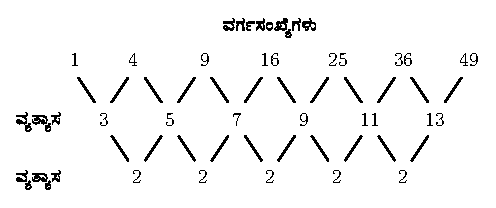
\includegraphics{src/figure/085a.eps}
\end{figure}

ideV riVti Gana saMKeyxgaLigU idu anavxyisutatxde.

\vfill\eject
\begin{figure}[h]
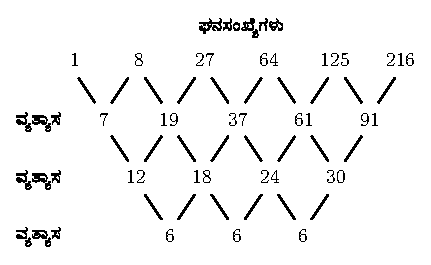
\includegraphics{src/figure/085b.eps}
\end{figure}

$41,80$ \;matutx\; $320$\; ralilx yAva eraDU saMKeyxgaLanunx kUDidarU vagaR\-saMKeyxyu barutatxde.
\begin{align*}
41+80 &=121=11^2\\
80+320 &= 400 = 20^2\\
320+41 &=361 = 19^2
\end{align*}
$41,80$\; matutx \;$320$\; I mUru saMKeyxgaLanunx kUDidaru vagaRsaMKeyx barutatxde. 
$$
41+80+320 = 441 = 21^2
$$

\begin{flushleft}
{\bf $\bf 142857$ idoMdu visamxyakArisaMKeyx}
\end{flushleft}

EkeMdare I saMKeyxyanunx $1$ riMda $6$ ravarege guNisidare datatxsaMKeyxyalilxruva aMkagaLu nidiRSaTxkarxmadalilx punarAvataRneyAgutatxde.
\begin{align*}
142857 \times 1 &= 142857&\\
142857 \times 2 &= 285714&\\
142857 \times 3 &= 428571&\\
142857 \times 4 &= 571428&\\
142857 \times 5 &= 714285&\\
142857 \times 6 &= 857142&\\
\text{Adare}\qquad 142857 \times 7 &= 999999&
\end{align*}

\vfill\eject
eraDu saMKeyxgaLa vagaRgaLa motatxvu matotxMdu saMKeyxya vagaRkekx sama.

\textbf{udAharaNege:}\qquad $3^2+4^2 = 5^2$

Adare eraDu saMKeyxgaLa GanagaLa motatxvu matotxMdu saMKeyxya Ganakekx sama\-nAgiralu sAdhayxvilalx.

eraDu saMKeyxgaLa GanagaLa motatxvu matetxraDu saMKeyxgaLa GanagaLa motatxkekx sama\-nAgirabahudu.
\begin{align*}
9^3+10^3 &= 1^3+12^3\\
15^3+9^3 &= 2^3+ 16^3
\end{align*}

eraDu saMKeyxgaLa GanagaLa motatxvu mototxMdu saMKeyxya Ganakekx samanAgiralu sAdhayxvilalx. Adare mUru saMKeyxgaLa GanagaLa motatxvu matotxMdu saMKeyxya Ganakekx sama.
\begin{align*}
3^3+4^3+5^3 &=6^3\\
1^3+6^3+8^3 &= 9^3
\end{align*}

